\chapter{Feedback and PID control}

In this lab you will be examining the effects of feedback on system
performance.  In particular, you will design a control, \(R_{C}\), for the
motor using the principles of PID control as shown in Figure~\ref{fig:PID}. It may be helpful to familiarize yourself with \textsf{Simulink} and \textsf{Matlab} (see e.g.\ Appendix~\ref{chap:MATLAB} and~\ref{chap:simulink}) before continuing with this lab.
\begin{figure}[htbp]
    \centering
    \begin{picture}(300,75)
        \put(-1,50){\(\hat\theta_{d}(s)\)}
        \put(22,53){\vector(1,0){13}}
        \put(40,53){\circle{7}}
        \put(47,53){\vector(1,0){13}}
        \put(30,57){+}
        \put(30,43){\_}
        \put(63,37){\framebox(85,33){\normalsize\(P+I \frac{1}{s}+Ds\)}}
        \put(150,53){\vector(1,0){20}}
        \put(175,53){\circle{7}}
        \put(180,53){\vector(1,0){20}}
        \put(203,37){\framebox(42.5,33){\Large\(\frac{k_{E}}{s(s+\frac{1}{\tau})}\)}}
        \put(247,53){\vector(1,0){30}}
        \put(280,50){\(\hat\theta(s)\)}
        \put(259,53){\line(0,-1){45}}
        \put(259,8){\line(-1,0){219}}
        \put(40,8){\vector(0,1){40}}
        \put(180,58){\(\hat u(s)\)}
    \end{picture}
    \caption{PID control system}\label{fig:PID}
\end{figure}%

where \( \tau \) is the \emph{motor constant} and \( k_E \) is the \emph{torque constant}. These constants vary slightly between motors but for our purposes we can use the approximate values of \( \tau \approx 0.036 \) and \( k_E \approx 229.16 \). For more information regarding the hardware for this lab see Appendix~\ref{chap:hardware}.

\section{Key Concepts}
In this lab, you will be implementing a PID controller into a closed loop
system. The main issue with open loop systems is that we only have
control over the reference trajectory, and therefore cannot account for
disturbances. Now, if we were to use feedback, we could attempt to control
the \emph{error} signal, which is the difference between the reference
trajectory (i.e.\ desired angle, or state of the motor) and the measured output.

A goal of a standard PID controller is to  tune the system to behave a certain
way by using various constants to correct the error signal. The three contstants
of a PID controller are \emph{Proportional}, \emph{Integral}, and \emph{Derivative}
controls.
\begin{itemize}
    \item \textbf{Proportional} control acts on the present value of the error signal. This is the most
          dominant of the three terms, but it can also leave some steady state error.
    \item\textbf{Integral} control accounts for the past values of error which is accumulated over time.
          This term will eliminate the steady state error that is left behind by the proportional control
          term, and also reduce rise time.
    \item \textbf{Derivative} control looks at the rate of change in the error signal, and attempts to
          correct for possible future values of error. For example, if the system is rapidly approaching
          its reference trajectory, (i.e.\ the error signal is rapidly approaching zero) the system will be
          able to slow down and avoid overshoot. Derivative control helps improve the settling time and
          stability of the system.
    \item Figure~\ref{fig:PIDExp} illustrates the concepts of a PID controller. You have some error
          signal, where the proportional term acts on the current state of the system, the integral term
          sums up all previous error, and the derivative term attempts to predict and control future error.

          \begin{figure}
              \centering
              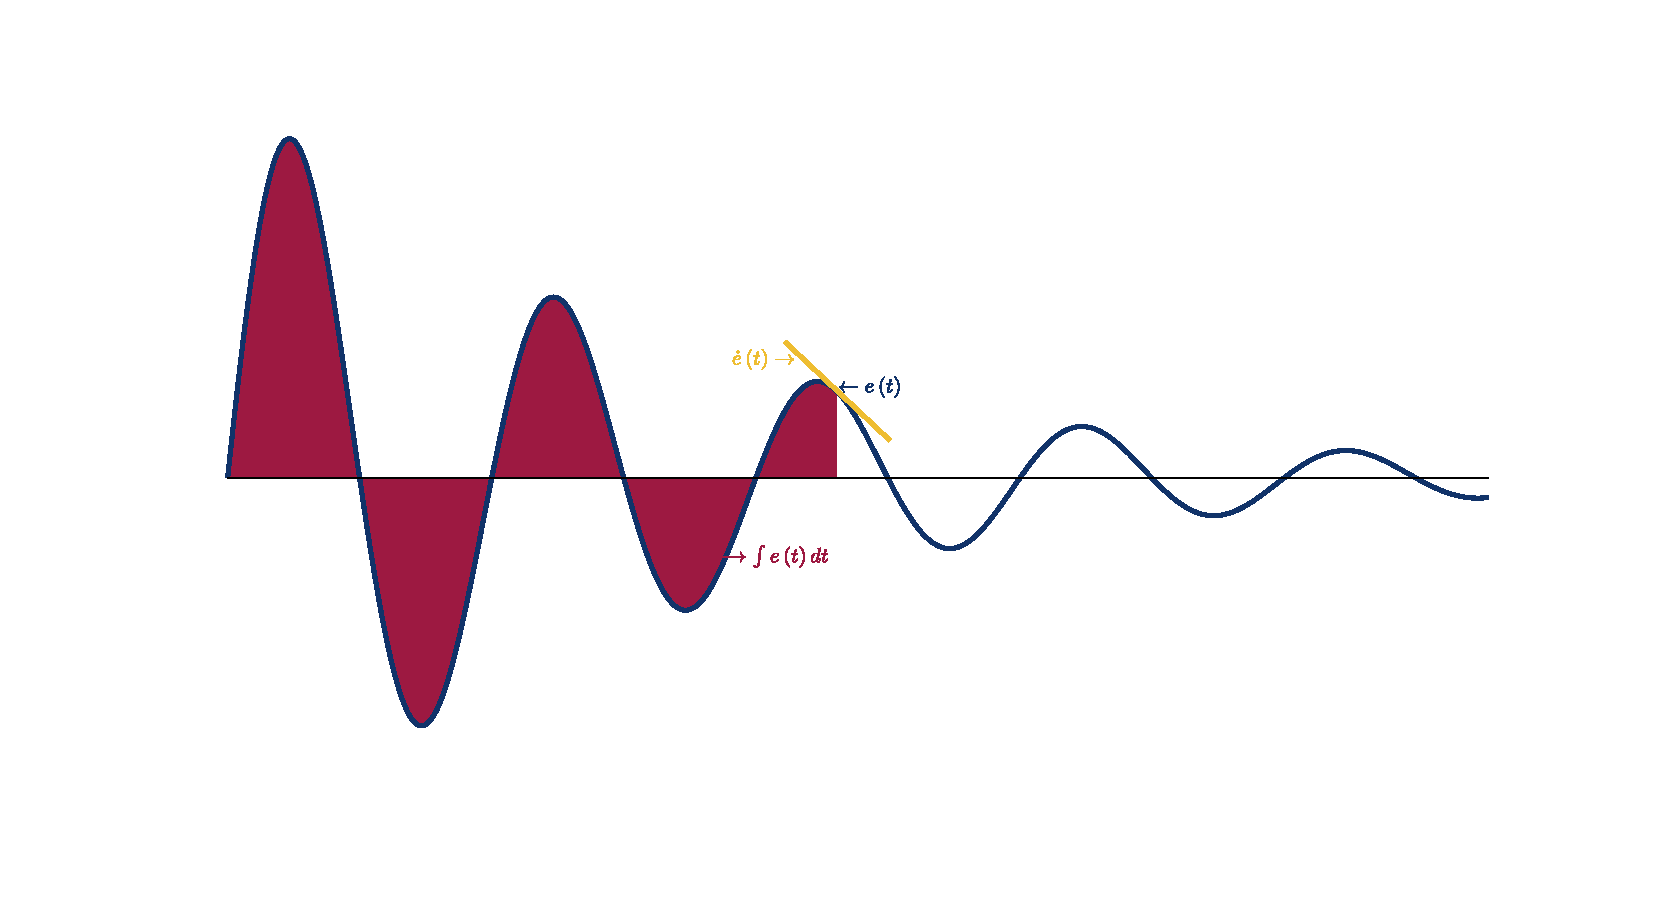
\includegraphics[width = 0.8\hsize]{pix/PIDSchematic.eps}
              \caption{Arbitrary error signal with a PID controller acting on it}\label{fig:PIDExp}
          \end{figure}
\end{itemize}

It is important to remember that when using  PID controllers, there will always be an element of
compromise within your system. For example, the ideal system will have a very low rise time, with
little to no steady state error or settling time, and no overshoot. However, this is very unrealistic in
the real world. If you were designing a highly precise robotic arm, you may need to tune your
controller in a way that there is practically no steady state error, but in order to do so, you will need to
have a higher rise time (i.e.\ the arm will move slowly, but it will go exactly where you need it). On
the other hand, you may have a system that requires a quick reaction time, for which you may need
to accept that there could be overshoot, or some steady state error.

You will also examine the concept of system types and their relation to PID controllers. Essentially,
systems can be type 0, 1, 2, etc \ldots A systems ``type'' determines its ability to track
the error on a given reference trajectory. For example, a system of type \(k \) can track
a reference trajectory with a bounded error for polynomials up to degree \(k \). We will see how the different terms from the PID controller transfer function affect the system type.

\section{Background Information}
\subsection{Definitions}
\begin{itemize}
    \item If our system output is \( y(t) \), then our \textbf{steady-state value} is defined by
          \[ \bar{y} = \lim_{t \to \infty}y(t) \]
          when the limit exists. Note that you may have to estimate this value by looking at output graphs.
    \item \textbf{Rise time} is the smallest time when the output reaches a certain percentage of its steady-state value. For our purposes, we will set this percentage to 90\%. That is,
          \[ t_r = \inf_t\{ t : y(t) \ge 0.9\bar{y} \} \]
    \item \textbf{Settling time} is the smallest time after which the output stays within a certain threshold \( \epsilon \) of the steady-state value. We will set \( \epsilon = 0.5 \), so that
          \[ t_s = \inf_{\delta}\{ \delta : |y(t) - \bar{y}| \le 0.5 \; \forall \; t \in [\delta, \infty)\} \]
    \item \textbf{Overshoot} is the maximum difference of the output \emph{over} the steady-state value. That is,
          \[ y_{os} = \sup_t \{y(t) - \bar{y}\} \]
    \item \textbf{Steady-state error} is the difference between the steady-state value and the reference trajectory. If our reference is \( r(t) \), then the steady-state error is defined by
          \[ \lim_{t \to \infty}|r(t) - y(t)| \]
\end{itemize}
\subsection{Transfer Functions}
The closed loop transfer function of the system in \ref{fig:PID} is given by

\begin{equation*}\label{eq:transfer}
    T(s)= \frac{R_{C}(s)R_{P}(s)}{1+R_{C}(s)R_{P}(s)}
\end{equation*}

where \( R_C = P + I\frac{1}{s} + Ds \) is the controller and \( R_P = \frac{\kappa_E}{s(s+\frac{1}{\tau})} \) is the plant. If using P, I, or D controls individually, the transfer function becomes

\begin{itemize}
    \item Proportional Control: \( R_C(s) = P \), so we get
          \[ T(s) = \frac{PR_P(s)}{1+PR_P(s)} = \frac{Pk_E}{s(s+\frac{1}{\tau}) + Pk_E} \]
    \item Derivative Control: \( R_C(s) = Ds \), so we get
          \[ T(s) = \frac{DsR_P(s)}{1+DsR_P(s)} = \frac{Dsk_E}{s(s+\frac{1}{\tau}+Dk_E)} \]
    \item Integral Control: \( R_C(s) = I\frac{1}{s} \), so we get
          \[ T(s) = \frac{I\frac{1}{s}R_P(s)}{1+I\frac{1}{s}R_P(s)} = \frac{Ik_E}{s^2(s+\frac{1}{\tau}+Ik_E)} \]
\end{itemize}

Consider the location of the closed loop poles in each of these cases. What condition is required on the constants \(P\), \(D\), and \(I\), respectively, such that the system is BIBO stable?

\section{Procedure}
You will be provided (e.g. through OnQ) a \textsf{Simulink} model that implements a PID controller. See Appendix~\ref{chap:simulink} for information on working with \textsf{Simulink}. Upon opening the model file, it should look similar to Figure~\ref{fig:model6}
\begin{figure}[H]
    \centering
    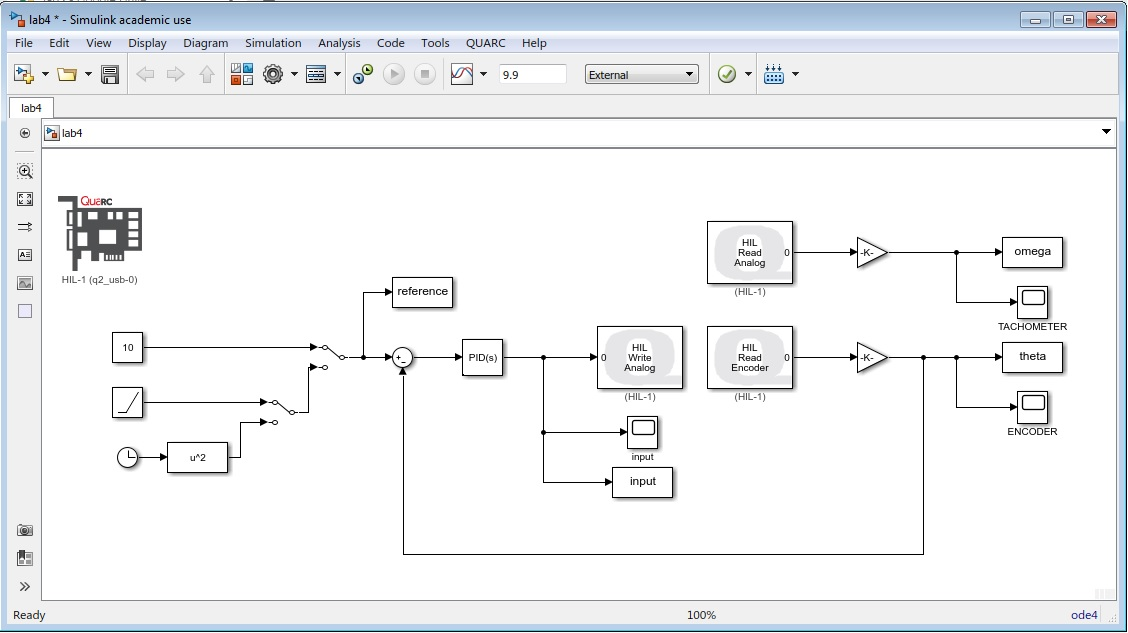
\includegraphics[width=0.6\hsize]{pix/performanceSpecificationModel4.jpg}
    \caption{\textsf{Simulink} model for a DC Servo Motor
        system}\label{fig:model6}
\end{figure}%

As shown in Figure~\ref{fig:PIDparameters}, the \verb|PID| block contains three parameters: \(P\) is the proportional gain, of the controller; \(I\) is the integral action parameter which is equal; the \(D\) term provides the derivative action.
\begin{figure}[H]
    \centering
    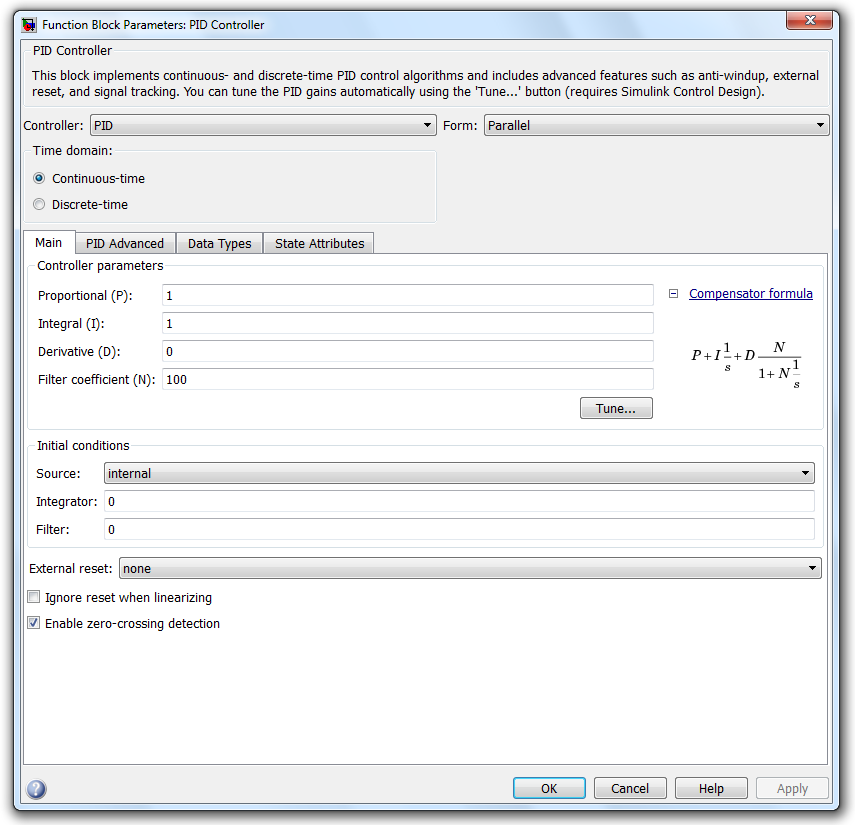
\includegraphics[width=0.6\hsize]{pix/PID.PNG}
    \caption{Screen shot of the \texttt{PID Controller} block}\label{fig:PIDparameters}
\end{figure}
Set the desired angle to 10 radians.  The desired input is entered as
shown in Figure~\ref{fig:model6} in the \verb|Constant| block. You should double check that the ``gain'' blocks for the encoder and tachometer (these are the triangle blocks leading into them) are
using the appropriate gain values from Table~\ref{tab:conversionFactors}. Also, check that the \verb|solver| in \verb|Configuration Parameters|
(\verb|Ctrl+E|) is set to \verb|ode 4|.

\begin{enumerate}
    \item \textbf{Proportional Term}\label{step:3} \begin{enumerate}
              \item Build and run the \textsf{Simulink} model using only the
                    proportional term (i.e., set \(I\) and
                    \(D\) to zero). Comment on the effects of using various values of \(P\).
                    In particular, comment on the overshoot, rise time, settling time, and the
                    steady-state error for different values of \(P\), and be sure to tabulate this data (a table in Excel is an efficient way to do this). Use at least three different values of \(P\).

              \item Keep \(D\) and \(I\) at 0 and increase the value of \(P\) so the
                    system oscillates about the desired value of 10 radians without (seemingly)
                    decreasing in magnitude. Print a copy of the encoder output at that value, and a copy when using a slightly lower value of \(P\). Why do higher \(P\) values increase the oscillation of the output? What is
                    happening to the location of the closed loop poles in equation~\eqref{eq:transfer}?

              \item Now reset your \(P\) value to the ``good'' value (i.e.\ not the value that makes
                    the system oscillate about 10 radians, but the value where you get a ``desirable'' response). Plot the error response of this system (i.e.\ the difference between input and output).
              \item Repeat the previous step but this time replace the constant input with linear input (i.e.\ disconnect the ``10'' block and connect the linear block). Plot the error response.
              \item Repeat the previous step but with the quadratic input (you may have to divide the quadratic term by 2 to prevent the encoder from going out of range).
              \item Based on the above error results, what is the type of the system when using only proportional control? Is this consistent with the BIBO stability criteria in~\eqref{eq:transfer}?
          \end{enumerate}

    \item \textbf{Derivative Term}\label{step:4}
          \begin{enumerate}
              \item Test various \(D\) values while keeping \(P\) constant (at the ``good'' value you found in the previous section), and comment on overshoot, rise time, settling time, and steady-state error. Again, tabulate this data, and decide on some ``good'' value of \(D\).
              \item Now, set \(P\) to 0 and repeat steps (c)-(e) from \ref{step:3} using only derivative control.
              \item Based on the above error results, what is the type of the system when using only derivative control? Is this consistent with the BIBO stability criteria in~\eqref{eq:transfer}?
          \end{enumerate}

    \item \textbf{Integral Term}\label{step:5} \begin{enumerate}
              \item Set your values of \(P\) and \(D\) to the values you found above, and test various \(I\) values.  Comment on the overshoot,
                    rise time, settling time, and steady-state error for these values of
                    \(I\), and tabulate the data.

              \item Now, set \(P\) and
                    \(D\) to zero and repeat steps (c)-(e) from \ref{step:3} using only integral control.
              \item Based on the above error results, what is the type of the system when using only integral control? Is this consistent with the BIBO stability criteria in~\eqref{eq:transfer}?
          \end{enumerate}

    \item \textbf{Using the PID Controller with a Complicated Input}

          Now we will consider a more complicated function input. To make things interesting, have the desired angle behave
          as four different functions on different intervals.  This can be achieved by
          preparing the \textsf{Simulink} model shown in Figure~\ref{fig:multiSwitch}\@.
          \emph{You do not need to use the exact same functions as shown in the figure}. Pick
          four functions that you think would be interesting.
          \begin{figure}[H]
              \centering
              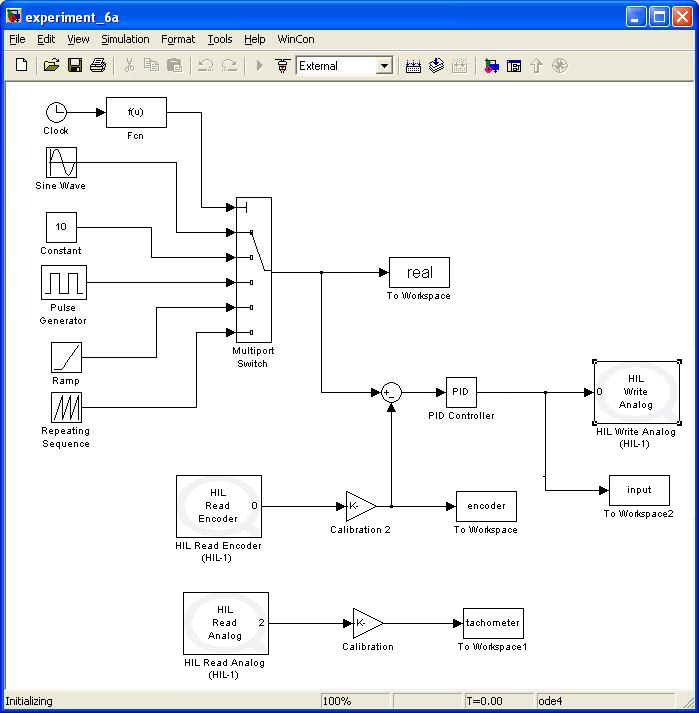
\includegraphics[width=0.6\hsize]{pix/lab6b.jpg}
              \caption{\textsf{Simulink} model for the implementation of multiple inputs and PID control}\label{fig:multiSwitch}
          \end{figure}%
          In this model, a number of possible sources have been introduced along with
          the switching logic.  The switching logic is based on the value of the
          function, \verb|4 sin(0.2*t)^{2}+1|.  This function, although arbitrary,
          assumes a value between 1 and 5 which is associated with ports 1 through 5 of
          the \verb|Multiport Switch| block.  The switching function is entered using
          the \verb|Fcn| block as indicated in Figure~\ref{fig:switchConfig}\@.
          \begin{figure}[H]
              \centering
              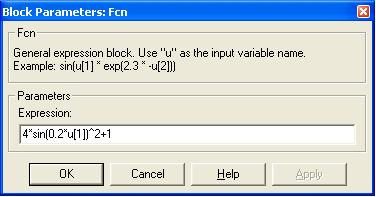
\includegraphics[width=0.6\hsize]{pix/fcnParameters.jpg}
              \caption{Configuration of the \texttt{Fcn} block for the implementation of multiple inputs and PID control}\label{fig:switchConfig}
          \end{figure}%
          \newpage
          \begin{enumerate}
              \item Run the system and prepare a plot comparing the angle and the desired angle
                    trajectory, making sure to note the values of the PID coefficients. You may have to tweak the PID values you found in previous sections in order to get a better trajectory.

                    When you have completed the lab, make sure you save your files in a convenient location (e.g.\ on some type of cloud storage).
          \end{enumerate}
\end{enumerate}

\section{Deliverables}
Prepare a brief write up describing what you learned from this lab. This does not need to be a formal report, but all material should be presented in a clear and logical manner, with concise descriptions where necessary. Include your answers to all the questions in the lab (these are the lettered sections in the procedure), as well as any requested plots.

%%% Local Variables: 
%%% mode: latex
%%% TeX-master: "lab-manual"
%%% End: 
